\documentclass[a4paper]{article}
\usepackage[top=1in,bottom=1in,left=1in,right=1in]{geometry}
\usepackage[utf8]{inputenc}
\usepackage{amsmath}
\usepackage{amssymb}
\usepackage{setspace}
\usepackage{color}
\usepackage{graphicx}
\usepackage{listings}
\usepackage{subcaption}
\usepackage{hyperref}

\setlength{\parskip}{1em}
\setlength{\parindent}{0pt}

\newcommand{\Rbb}{\mathbb{R}}
\newcommand{\Expect}{\mathbb{E}}
\newcommand{\Var}{\text{Var}}
\newcommand{\Cov}{\text{Cov}}
\DeclareMathOperator*{\argmin}{arg\,min}
% \DeclareMathOperator*{\sup}{sup}

\title{Sensitivity in BNP}
\author{Runjing (Bryan) Liu}
\date{\today}

\begin{document}
\maketitle
\tableofcontents
\newpage
\section{Introduction}

We examine the sensitivity of clustering results from fitting a
Bayesian non-parametric model to various perturbations of
the Dirichlet stick-breaking process.
We approximate the true posterior using variational methods, and compute
sensitivities to the prior using formulae from \cite{giordano_2017}.
We are particularly interested in examining how the ``number of posterior
clusters" changes when the prior is perturbed. We experiment with the sensitivity
of BNP by fitting the model on the iris dataset
\cite{iris_dataset}, which
involves measurements on three flower species.

We also compare the results of this Bayesian approach with a frequentist approach,
which uses bootstrap sampling to choose the number of clusters. Finally, we
show how the sensitivity computations used for computing prior sensitivity can
also be used to approximate the bootstrap sampling in this frequentist approach.


\section{Data}
We use the iris dataset \cite{iris_dataset}, which contains 150 observations of
three different types
of irises: Setosa, Versicolour, and Virginica. We use measurements of their
sepal length, sepal width, petal length, and petal width to cluster the data with
the goal of recovering the three species. The data is shown visually in figure \ref{fig:iris_data}.

\begin{figure}[h!]
	\centering
	\begin{subfigure}[t]{0.4\textwidth}
		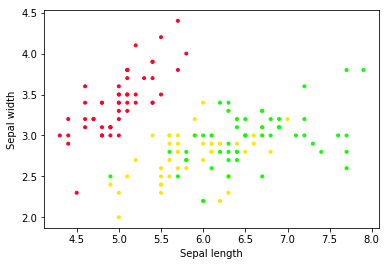
\includegraphics[width = \textwidth]{./data_figs/iris_data.png}
		\subcaption{}
	\end{subfigure}
  \begin{subfigure}[t]{0.4\textwidth}
    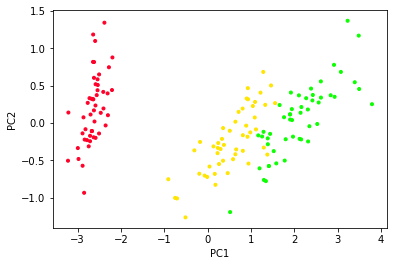
\includegraphics[width = \textwidth]{./data_figs/pca_iris_data.png}
    \subcaption{}
  \end{subfigure}
	\caption{Visualization of the iris dataset in two dimensions. Points are colored by their
  true species: red, Setosa; yellow, Versicolour;
  and green, Virginica. (a) The sepal length against sepal width. (b) The
  the data projected onto the first two principal components after running PCA.
  }
	\label{fig:iris_data}
\end{figure}

\section{Model}
Let $y_{n}\in \mathbb{R}^4$ be the four measurements
(sepal length, sepal width, petal length, and petal width)
for flower $n$, and $n = 1, ..., 150$.

Now, let $z_n$ denote the cluster (i.e. the species, which we treat as unknown)
to which flower $n$ belongs.
Each cluster has mean $\mu_k\in \mathbb{R}^4$  and covariance $\Sigma_k \in \mathbb{R}^{4\times 4}$.
Our data generating process is then
\begin{align}
	y_n | z_n \sim \mathcal{N}\Big(\sum_{k=1}^\infty \mathbb{I}\{z_n = k\} \mu_k \;,
              \; \sum_{k=1}^\infty \mathbb{I}\{z_n = k\} \Sigma_k\Big),
	\quad n = 1, ..., N
\end{align}
Note that we allow for an infinite number of clusters. The next section describes
the Bayesian non-parametric prior that makes this possible.

\subsection{Our prior}
We place priors on $\mu_k$, $\Sigma_k$, and $z_n$. \par

We use a Dirichlet stick breaking process \cite{dp_prior} as our prior on the cluster components
weights $\pi$, and draw $z_n$ from a multinomial with said weights:
\begin{align}
	\pi &\sim \text{GEM}(\alpha) \label{eq:GEM} \\
	 z_n &\sim \text{Multinomial}(\pi), \quad n = 1..., 150
\end{align}

We can write out equation~\ref{eq:GEM} more explicitly as,
\begin{align}
  \nu_k | \alpha &\sim Beta(1, \alpha) \quad k = 1, .., \infty \label{eq:beta_sticks}\\
  \pi_k | \nu &= \nu_k \prod_{j=1}^{k-1} (1 - \nu_j) \label{eq:stick_breaking}
\end{align}
so posterior inference on the cluster proportions amounts to doing
posterior inference on the sticks $\nu_k$'s.

The other parameters have priors:
\begin{align}
	\mu_k &\sim \mathcal{N}(0, \sigma^2 I_{4\times 4}), \quad k = 1, 2, 3 ... \\
	\Sigma_k &\sim \text{Inv.Wishart}(d, V), \quad k = 1, 2, 3 ...
\end{align}


\section{Variational approximation}
A true BNP representation would take $K = \infty$, but in order to make a computationally feasible
algorithm we truncate $K$ at a value large enough so that many clusters are essentially unoccupied in
the approximate posterior. The variational approximation is
\begin{align}
q(\nu, \mu, \Sigma, z) & =
\Big\{\prod_{k=1}^{K}q\left(\nu_{k}\right)\delta\left(\mu_{k}\right)\delta\left(\Sigma_{k}\right)\Big\} \prod_{n=1}^{150}q\left(z_{n}\right),
\end{align}
where $\delta\left(\cdot\right)$ denotes a point mass at a parameterized
location, $q\left(\nu_{k}\right)$ is a logitnormal distribution, and $q\left(z_{n}\right)$
is a multinomial distribution.

In the future, we shall let $\eta$ represent the variational parameters be the parameters of the variational distribution
(the mean variance of the logitnormal, the locations of the point masses, etc.).

With this variational approximation, we seek
\begin{align}
\eta^* = \argmin_{\eta} KL\Big(q_\eta(\nu, \mu, \Sigma, z) \big\| p(\nu, \mu, \Sigma, z | y)\Big) \label{eq:kl_objective}
\end{align}

\subsection{The fit}
We show the results of our fit in figure \ref{fig:lucky_fit}. We again plot the datapoints
projected along the first two principal components. The black points are the cluster
centroids $\mu_k$, and the ellipses represent the region within $3\Sigma_k$ of the centroid.
The points are colored by the cluster belonging, $z_n$. We see that for this particular fit, we
almost exactly recover the true species (cf. \ref{fig:iris_data}b).

\begin{figure}[h!]
	\centering
	\begin{subfigure}[t]{0.4\textwidth}
		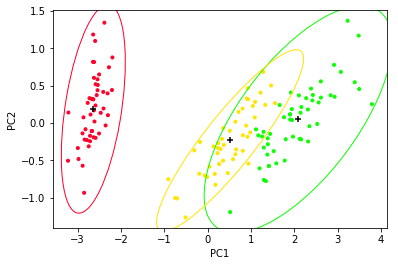
\includegraphics[width = \textwidth]{./data_figs/iris_lucky_clustering.png}
		\subcaption{}
	\end{subfigure}
  \begin{subfigure}[t]{0.3\textwidth}
    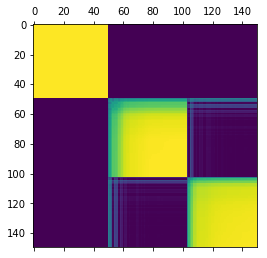
\includegraphics[width = \textwidth]{./data_figs/iris_lucky_clustering_coclust_mat.png}
		\subcaption{}
  \end{subfigure}
	\caption{(a) The data plotted in PC space along the first two principal components, and colored by
	cluster belonging in the model fit.
	(b) The co-clustering matrix from the fit. }
	\label{fig:lucky_fit}
\end{figure}

However, our optimization objective, equation \ref{eq:kl_objective} is highly non-convex. Thus,
it is very likely to land in different local optima, depending on the the initialization. The results
of six different restarts are shown in figure \ref{fig:pca_bnp_multiple_restarts}, and we see that
depending on the initialization, the Versicolour and Virginica clusters are often mixed together, though
the Setosa cluster seems robust across random restarts. Hence, this suggests that in addition to considering
stability to model assumptions (e.g the prior, the likelihood), we must also consider stability to the
algorithm, in this case, the robustness of our results to random restarts.

\begin{figure}[h!]
	\centering
	\begin{subfigure}[t]{0.6\textwidth}
		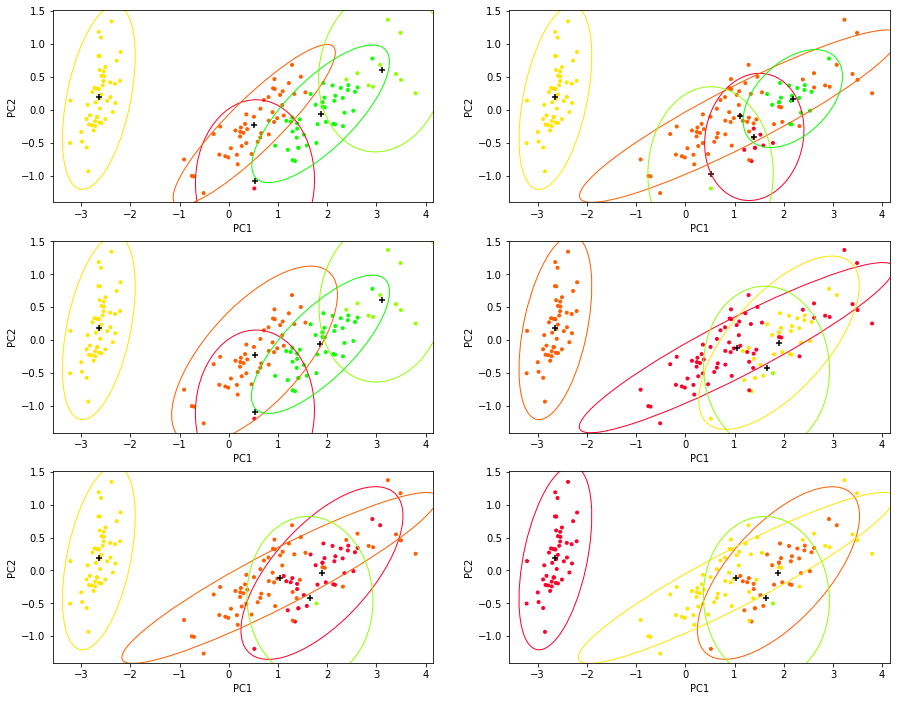
\includegraphics[width = \textwidth]{./data_figs/pca_bnp_multiple_clustering.png}
	\end{subfigure}
  \begin{subfigure}[t]{0.39\textwidth}
    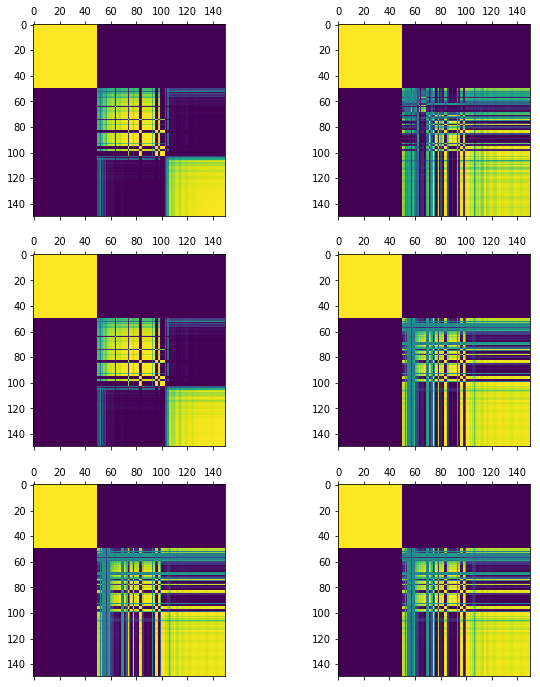
\includegraphics[width = \textwidth]{./data_figs/pca_bnp_multiple_clustering_coclust_mat.png}
  \end{subfigure}
	\caption{The results of fitting the same model but from multiple restarts. Colors represent
	cluster belongings in the model fit. }
	\label{fig:pca_bnp_multiple_restarts}
\end{figure}

In the sequel, we shall compare the results from this variational Bayesian method to a
frequentist approach. We shall also consider a MCMC approach ({\color{red} TODO}), to see if this result
of sensitivity to random restarts is unique to doing variational Bayes.

\section{Parametric Sensitivity}
We first consider the sensitivity to some prior parameter, $\alpha$. Our posterior depends on $\alpha$ through
the prior, $p_{\alpha}(\theta | y) \propto p(y |\theta) p_\alpha(\theta)$. (In this notation, we have absorbed the
quantities of interest into $\theta$; in our case specifically, $\theta$ contains the centroids $\mu$, the covariances
$\Sigma$, the sticks $\nu$, and the cluster belongings $z_n$). Suppose we are interested in the mean of some posterior
quantity, $E_{p_{\alpha}(\theta | y)}[g(\theta)]$. Our measure of sensitivity is its derivative with respect to $\alpha$:
\begin{align}
  S_\alpha := \frac{d}{d\alpha}E_{p_{\alpha}(\theta | y)} \big[g(\theta)\big]
\end{align}
Should we have chosen a different $\alpha$, say $\alpha + \epsilon$, then we can approximate
$E_{p_{\alpha + \epsilon}(\theta | y)} \big[g(\theta)\big]$ with
\begin{align}
  E_{p_{\alpha + \epsilon}(\theta | y)} \big[g(\theta)\big] = E_{p_{\alpha}(\theta | y)}[g(\theta)] +
    S_\alpha \cdot \epsilon + \mathcal{O}(\epsilon^2)
\end{align}
But since $p(\theta | y)$ is intractable, we replace the expectations over the posterior with expectations over
our variational approximation. Specifically, let $\eta^*(\alpha) =
\argmin_\eta KL(q_\eta\left(\theta\right) \| p_{\alpha}(\theta | y))$, and note the
dependence of the optimal variational parameters $\eta^*$ on $\alpha$. Then we approximate
\begin{align}
  \frac{d}{d\alpha}E_{p_{\alpha}(\theta | y)} \big[g(\theta)\big] \approx
  \frac{d}{d\alpha}E_{q_{\eta^*(\alpha)}} \big[g(\theta)\big] =: S_\alpha^q
\end{align}
And we can approximate
\begin{align}
  E_{p_{\alpha + \epsilon}(\theta | y)} \big[g(\theta)\big] \approx E_{q_{\eta^*(\alpha + \epsilon)}} \big[g(\theta)\big] = E_{q_{\eta^*(\alpha)}}\big[g(\theta)\big] +
    S_\alpha^q \cdot \epsilon + \mathcal{O}(\epsilon^2)
    \label{eq:our_approximation}
\end{align}

Following \cite{giordano_2017},  we compute $S^q_\alpha$ as:
\begin{align}
  S^q_\alpha &=
    g_\eta H^{-1} f_\eta \label{eq:vb_sensitivty}
\end{align}
where
\begin{align}
  g_\eta &= \frac{\partial}{\partial \eta}\Big\rvert_{\eta = \eta^*} E_{q_{\eta}} \big[g(\theta)\big] \\
  H &= \frac{\partial^2}{\partial^2\eta}\Big\rvert_{\eta = \eta^*} KL(q_\eta\left(\theta\right) \| p(\theta | y)) \\
  f_\eta &= \frac{\partial^2}{\partial \alpha \partial \eta}\Big\rvert_{\eta = \eta^*, \alpha = \alpha} E_{q_{\eta}} \big[p_\alpha(\theta)\big]
\end{align}

\subsection{Results}
The prior parameter we consider here is the choice of $\alpha$ for the DP prior (see equation \ref{eq:beta_sticks}).
We chose $\alpha = 4.0$, and we evaluate the sensitivity of posterior results to this choice of
$\alpha$. We perturb $\alpha$ for a range of $\epsilon$. After each perturbation,
we re-run the optimization procedure. These new fits after each epsilon perturbation are shown in
figure \ref{fig:vary_alpha_fits}. When perturbing $\alpha$ between with an $\epsilon$ between
-3, and 1, the fits all look similar. When $\epsilon > 1$, we see that more clusters start to appear.

\begin{figure}[h!]
	\centering
	\begin{subfigure}[t]{0.6\textwidth}
		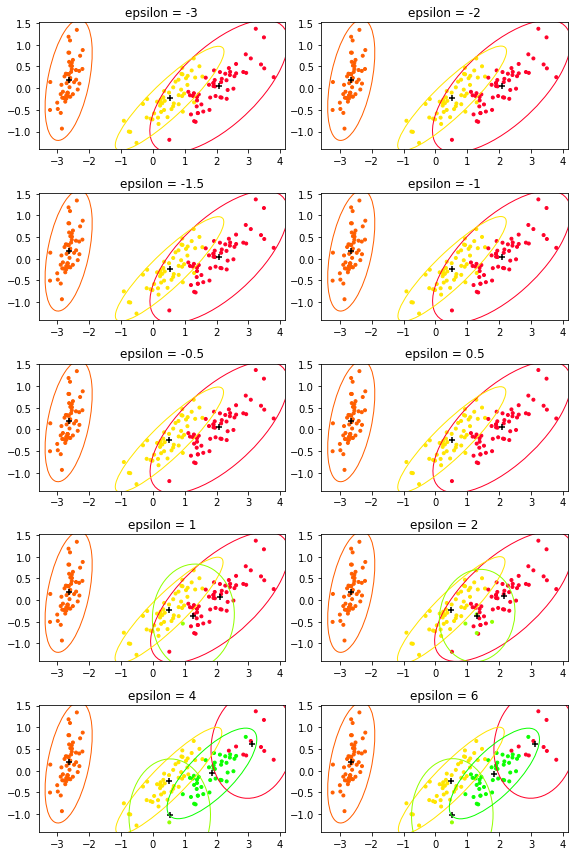
\includegraphics[width = \textwidth]{./parametric_sensitivity_figs/sensitivity_datapoints.png}
	\end{subfigure}
	\caption{The fits over a range of $\epsilon$ perturbations to the DP prior $\alpha$. }
	\label{fig:vary_alpha_fits}
\end{figure}

The fact that more clusters appear as we increase $\alpha$ is expected from the structure
of the stick breaking process: recall that the sticks are distributed $\text{Beta}(1, \alpha)$,
so larger $\alpha$ puts more prior mass on smaller sticks. We wish to evaluate the
sensitivity of the fits to changes in $\alpha$, and do so efficiently without having to
do expensive re-optimizations. To do so, we use the linear approximation described
above. We compare how well the linear approximation can predict the changes in the fits after perturbing $\alpha$.
In figure \ref{fig:vary_alpha_cocluster_weights}, the posterior means that we compared
are the the posterior co-clusterings $\sum_{k} q(z_{nk})q(z_{mk})$ and the posterior weights $\pi_k$.

\begin{figure}[h!]
	\centering
	\begin{subfigure}[t]{0.45\textwidth}
		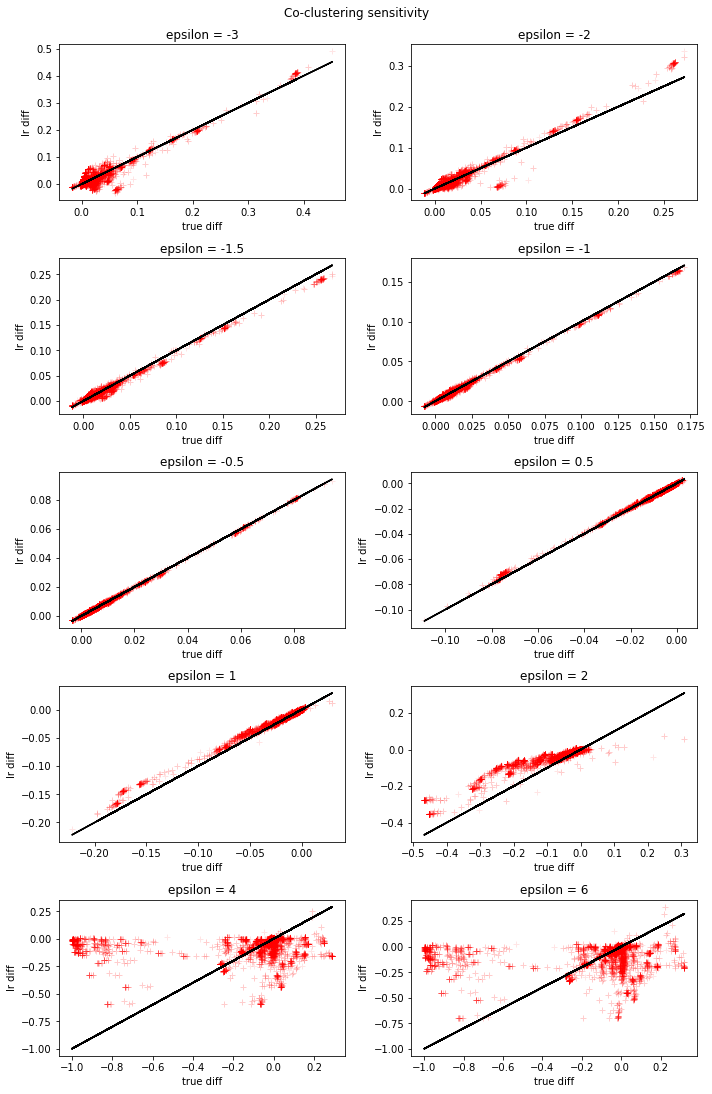
\includegraphics[width = \textwidth]{./parametric_sensitivity_figs/cocluster_sensitivity.png}
	\end{subfigure}
	\quad
	\begin{subfigure}[t]{0.45\textwidth}
		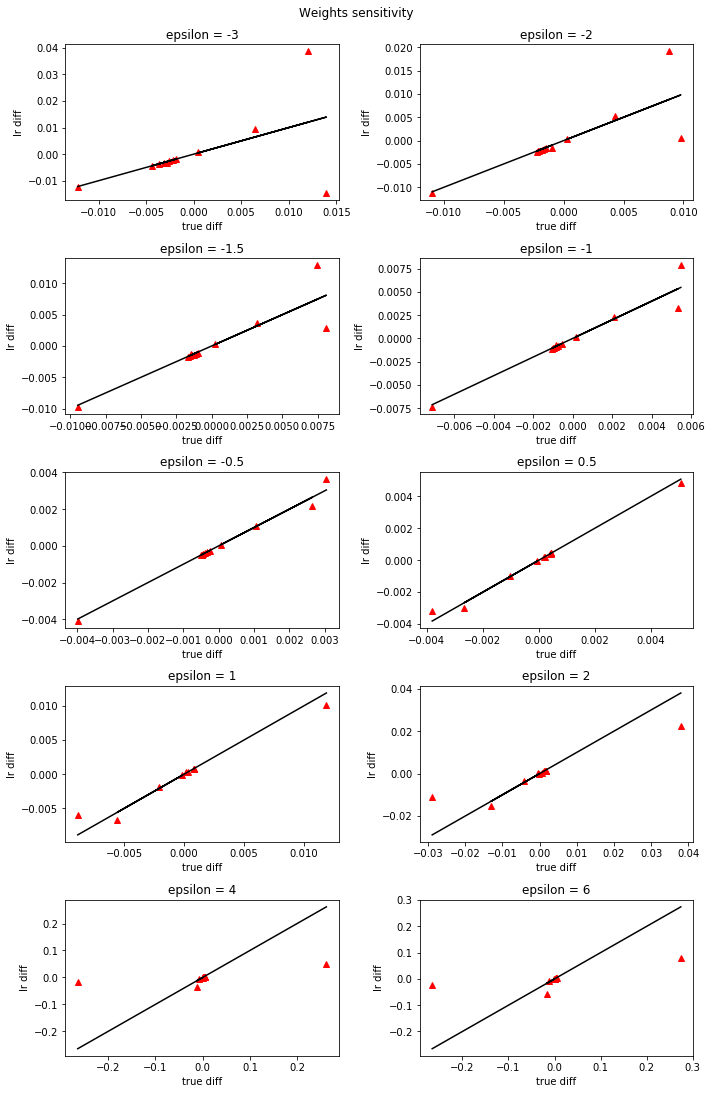
\includegraphics[width = \textwidth]{./parametric_sensitivity_figs/weight_sensitivity.png}
	\end{subfigure}
	\caption{The accuracy of our linear approximation over a range of perturbations $\epsilon$.
  For each plot, the $y$-axis is the difference predicted by the linear approximation,
  while on the $x$-axis is the difference observed after re-optimizing with the perturbed $\alpha$.
  In (a) we examine our predictions for the change in co-clusterings, $E_q[\sum_k z_{nk}z_{mk}] = \sum_{k} q(z_{nk})q(z_{mk})$,
	for $n, m = 1, ..., 150$; in (b) we examine our
	predictions for the change in cluster weights $E_{q}[\pi_k]$, for $k = 1, ..., K$.  }
	\label{fig:vary_alpha_cocluster_weights}
\end{figure}

As expected, the linear sensitivity works best when $\epsilon$ is small. For this particular
example, the linear sensitivity gave a good approximation when $\epsilon$ was between -2 and 2;
when $\epsilon$ is large, the linear response under-estimates the true differences.

Another posterior quantity of interest is the ``number of clusters.''
In the BNP set-up we have an infinite number of latent clusters (or a large
finite number of clusters in the approximation). Hence, we define the
``number of clusters'' as the the expected number of clusters that would manifest
in a draw from the posterior predictive distribution. That is, in this setting, we define the
``number of clusters'' as
\begin{align}
  \hat K &= \mathbb{E}_{z_n, \pi_k | y} \Big[\sum_{k = 1}^\infty \mathbb{I}\{\text{at least one $z_n = k$}\}\Big]\\
    &= \mathbb{E}_{\pi_k | y} \Big[\sum_{k = 1}^\infty \{1 - (1 - \pi_k)^{150}\} \Big]
		\label{eq:num_clusters}
\end{align}

We then approximate this quantity by replacing the expectation over the true posterior
with the expectation over the variational distribution, and replace the sum from 1 to infinity
with a sum from 1 to the number of clusters in the variational approximation.

With this expectation, we can again apply the linear approximation to evaluate sensitivities
with respect to the DP prior parameter. In figure \ref{fig:vary_alpha_e_num_clusters},
we compare the expected number of clusters obtained from re-optimizing
to the expected number of clusters predicted by our linear approximation.
The using the linear approximation gives similar results to re-optimizing: we find that the expected number of
clusters is rather sensitive to our choice of $\alpha = 4.0$, and the growth in
the expected number of clusters appears linear with $\alpha$ for $\alpha$ between 2 and 6;
the growth seems to decrease when $\alpha$ is larger.

\begin{figure}[h!]
	\centering
	\begin{subfigure}[t]{0.45\textwidth}
		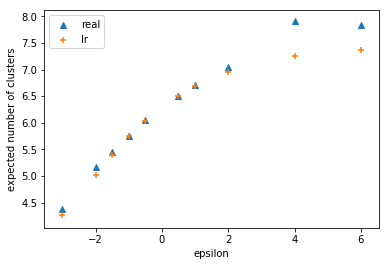
\includegraphics[width = \textwidth]{./parametric_sensitivity_figs/e_num_clusters_sensitivity.png}
	\end{subfigure}
	\caption{The expected number of posterior clusters after re-optimization (blue) with new
	$\alpha$'s, and the value predicted by the linear approximation (orange). }
	\label{fig:vary_alpha_e_num_clusters}
\end{figure}

% The linear approximation seems very accurate for a range of $\epsilon$ between -2 and 2,
% and hence provides an efficient alternative to evaluating prior sensitivities.

The linear approximation is also much faster than re-optimizing {\color{red} TODO: timing results}

\newpage

\section{Functional sensitivity}
\subsection{Functional perturbations and the influence function}
We go beyond the parametric perturbations of the previous section, and consider changing the functional
form of the prior itself. Suppose we perturbed the original prior $p_0(\theta)$ with some non-negative integrable
function $u(\theta)$,
\begin{align}
  p_\alpha(\theta) = \frac{p_0(\theta) + \alpha u(\theta)}{\int [p_0(\theta') + \alpha u(\theta')] d\theta'}
\end{align}
Then by equation~\ref{eq:vb_sensitivty}, the sensitivity of $E_{q_{\eta^*(\alpha)}} \big[g(\theta)\big]$ to $\alpha$ is
given by
\begin{align}
  S_u^q := \frac{d}{d\alpha} E_{q_{\eta^*(\alpha)}} \big[g(\theta)\big] = g_\eta H^{-1} \frac{\partial}{\partial\eta}E_{q_\eta}\Big[ \frac{u(\theta)}{p_0(\theta)}\Big]\Big|_{\eta = \eta^*(\alpha)}
  \label{eq:fun_sensitivity}
\end{align}
If we view $E_{q_{\eta^*(\alpha)}} \big[g(\theta)\big]$ as a functional of $u(\theta)$, then $S_u^q$ is a Gateaux derivative
of $E_{q_{\eta^*(\alpha)}} \big[g(\theta)\big]$ in the direction of $u(\theta)$.

We also define the influence function $I(\theta)$ that characterizes the relationship of $S_u^q$ to $u$. Specifically, it satisfies
$S_u^q = \int I(\theta) u(\theta) d\theta$, and reading from equation~\ref{eq:fun_sensitivity}, we get that
\begin{align}
  I(\theta) := \Big(\frac{q_\eta (\theta)}{p_0(\theta)}\Big) \cdot
  g_\eta H^{-1} \frac{\partial}{\partial \eta} \Big[\log q_\eta(\theta)\Big]
\end{align}

In our case, we consider perturbing our DP process prior. Recall that the sticks $\nu_k$ were drawn iid
from a $Beta(1, \alpha)$ distribution. If we perturb each stick by the same perturbation $u(\cdot)$, then the sensitivity is given by
\begin{align}
S_u^q &=
g_\eta H^{-1} \sum_{k = 1}^K \frac{\partial}{\partial \eta} E_{q_\eta(\nu_k)}\Big[\frac{u(\nu_k)}{p_0(\nu_k)} \Big]
\end{align}
where $p_0(\nu_k)$ is the $Beta(1, \alpha)$ pdf. We can now define the {\itshape total} influence function as
\begin{align}
I(\cdot) = g_\eta H^{-1} \sum_{k = 1}^K \frac{q_{\nu_k; \eta}(\cdot)}{p_0(\cdot)}\frac{\partial\log q_{\nu_k; \eta}(\cdot)}{\partial \eta}
\label{eq:total_influence}
\end{align}
where $q_{\nu_k; \eta}$ is the variational approximation specifically for the $k$th stick.

\subsubsection{Results}

In figure \ref{fig:influence_on_weights}, we plot the total influence on the posterior cluster weights,
$\pi_k$. We note that the influence functions deviate furthest from zero at values close to 1.
In other words, the posterior cluster weights are most sensitive to
perturbations that bias the prior stick distribution towards
larger sticks. Moreover, the influence on the first four cluster weights are positive, while the
rest are negative. This is reasonable by examining the stick breaking formula,
equation \ref{eq:stick_breaking}; making the sticks larger encourages the first sticks
to be large, with less length left over for later sticks. Finally, the weights with the largest
influence functions are those corresponding to clusters 0 and 3,
which are the Versicolour and the Virginica clusters in figure \ref{fig:lucky_fit}.
These were the two clusters that our model had a hard time differentiating.
The clear Setosa cluster corresponded to cluster 1, and this weight had a small influence function,
and hence we expect it to be robust to prior perturbations.


\begin{figure}[h!]
	\centering
	\begin{subfigure}[t]{0.6\textwidth}
		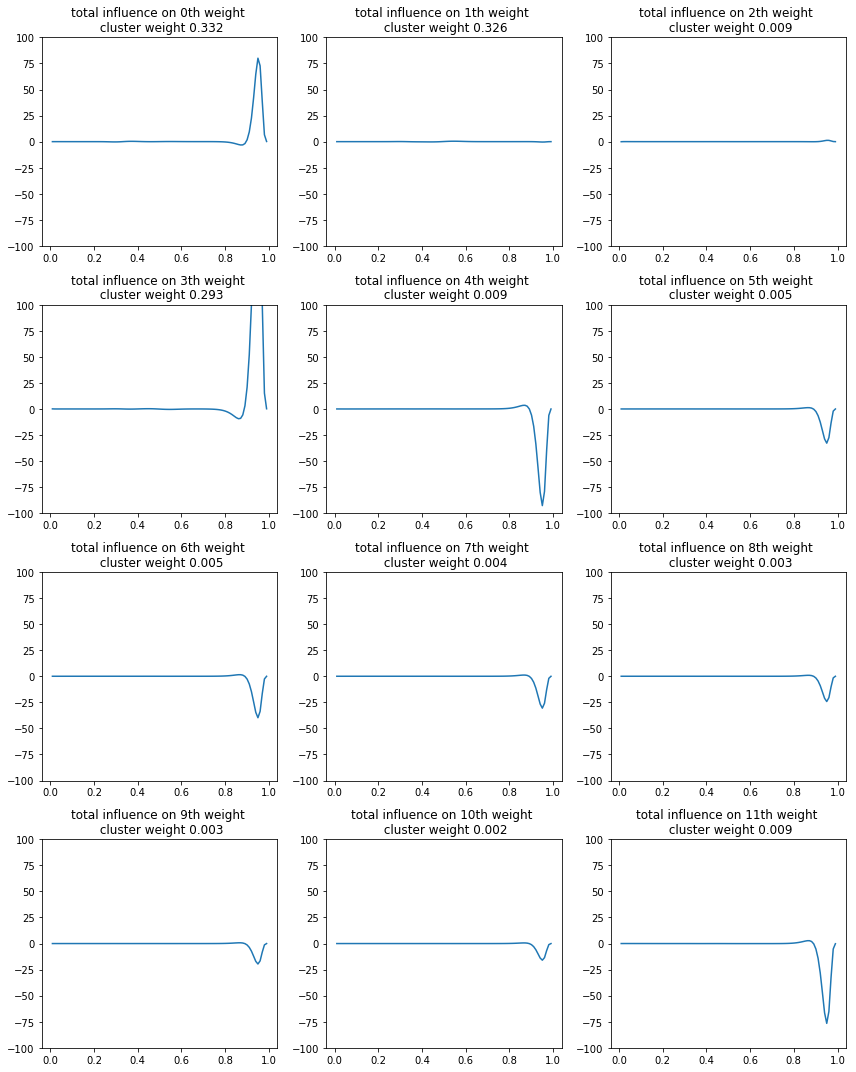
\includegraphics[width = \textwidth]{./functional_sensitivity_figs/influence_on_weights.png}
	\end{subfigure}
	\caption{The {\itshape total} influence function on the posterior means of the cluster weights $\pi_k$, $k = 0, ..., 11$.
	Also noted are the actual posterior mean of the cluster weights. $k = 0$ corresponds to the Virginica (green) cluster
	in figure \ref{fig:lucky_fit}; $k = 1$ the Setosa (red) cluster; and $k = 3$ the Versicolour (yellow) cluster. }
	\label{fig:influence_on_weights}
\end{figure}


In figure \ref{fig:influence_fun_on_num_clusters}, we plot the influence function on the expected number of
posterior clusters $\hat K$ (recall, as defined in equation \ref{eq:num_clusters}). The influence of the
{\itshape individual} sticks on $\hat K$ is shown in figure \ref{fig:influence_fun_on_num_clusters}a,
and we observe that the third stick has by far the greatest influence ({\color{red} why?}).
In figure \ref{fig:influence_on_num_clusters}b, we plot the {\itshape total} influence,
which is the sum of the individual influence functions.

\begin{figure}[h!]
	\centering
	\begin{subfigure}[t]{0.6\textwidth}
		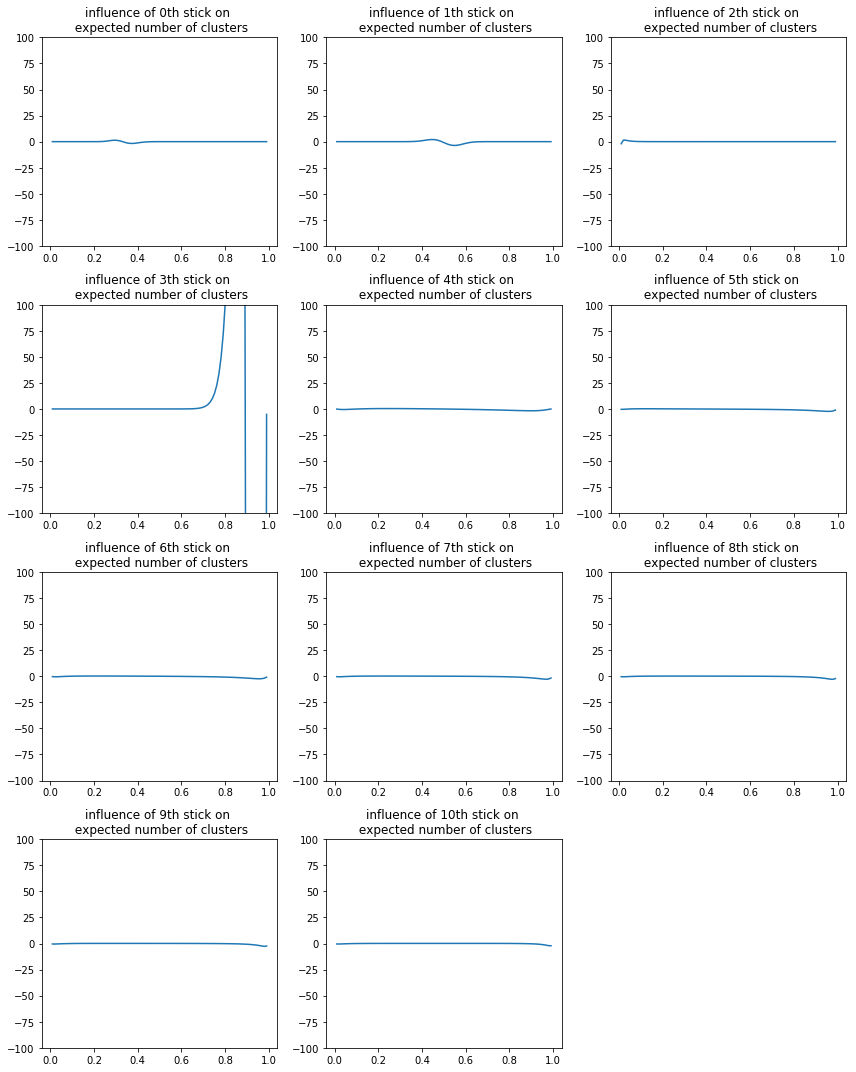
\includegraphics[width = \textwidth]{./functional_sensitivity_figs/influence_on_num_clusters.png}
		\subcaption{The influence function of {\itshape individual} sticks on the expected
		number of posterior clusters.}
	\end{subfigure}\\
	\quad \\
	\begin{subfigure}[t]{0.5\textwidth}
		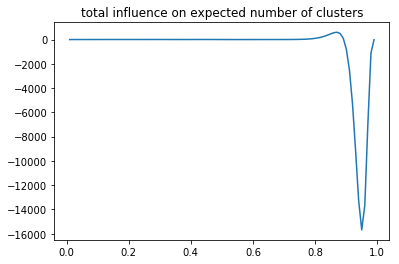
\includegraphics[width = \textwidth]{./functional_sensitivity_figs/total_influence_on_num_clusters.png}
		\subcaption{The {\itshape total} influence function on the expected
		number of posterior clusters.}
	\end{subfigure}
	\caption{Influence on the expected number of clusters (as defined in equation \ref{eq:num_clusters}). }
	\label{fig:influence_fun_on_num_clusters}
\end{figure}

% \begin{figure}[h!]
% 	\centering
% 	\begin{subfigure}[t]{0.6\textwidth}
% 		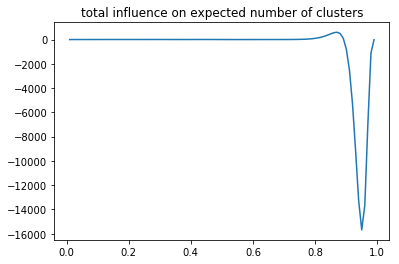
\includegraphics[width = \textwidth]{./functional_sensitivity_figs/total_influence_on_num_clusters.png}
% 	\end{subfigure}
% 	\caption{The {\itshape total} influence function on the expected
% 	number of posterior clusters (as defined in equation \ref{eq:num_clusters}).}
% 	\label{fig:total_influence_on_num_clusters}
% \end{figure}

Next, we consider two different functional perturbations, and examine their effect
on $\hat K$. The first perturbation is shown in
figure \ref{fig:influence_on_num_clusters}a,
where we placed a perturbation with mass corresponding to the positive part
of the influence function from figure \ref{fig:influence_fun_on_num_clusters}b. We
vary the size of the perturbation $\epsilon$, that is, the we perturb the prior with
$\epsilon \cdot u(x)$, and compare the predictions of the linear approximation against
the true value from re-optimizing with this perturbed prior. The results are shown in figure
\ref{fig:influence_on_num_clusters}b. We see in both the linear approximation and
after re-optimizing that the expected number of posterior clusters increase with $\epsilon$, as
expected, and the linear approximation is best with small $\epsilon$.

The second perturbation examined is shown in figure \ref{fig:influence_on_num_clusters2}a,
where we placed a perturbation on the negative part of the influence function. This time,
the $\hat K$ decreases with $\epsilon$, as expected, and
this behavior is manifest in both the linear approximation and after re-optimizing.

\begin{figure}[h!]
	\centering
	\begin{subfigure}[t]{0.4\textwidth}
		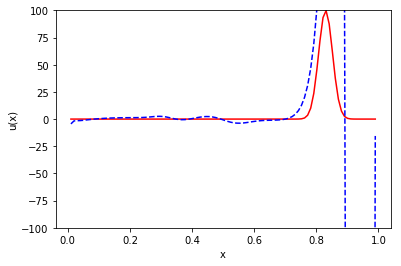
\includegraphics[width = \textwidth]{./functional_sensitivity_figs/pert1.png}
		\subcaption{}
	\end{subfigure}
	\begin{subfigure}[t]{0.4\textwidth}
		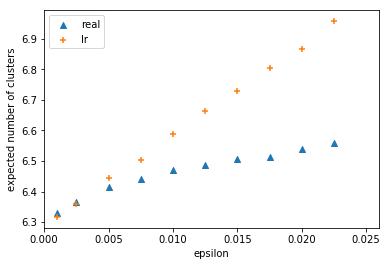
\includegraphics[width = \textwidth]{./functional_sensitivity_figs/vary_epsilon_e_num_clust.png}
		\subcaption{}
	\end{subfigure}
	\caption{(a) The functional perturbation $u(x)$ that we applied to the prior stick distribution in solid red. The dashed
	blue line is the total influence on the expected number of clusters. (b) Comparing the expected number of clusters gotten from
	re-optimizing with the perturbation $u(x)$ (blue triangles) against the prediction of linear response (orange +), as
	the size of the perturbation $\epsilon$ is varied}
	\label{fig:influence_on_num_clusters}
\end{figure}

\begin{figure}[h!]
	\centering
	\begin{subfigure}[t]{0.4\textwidth}
		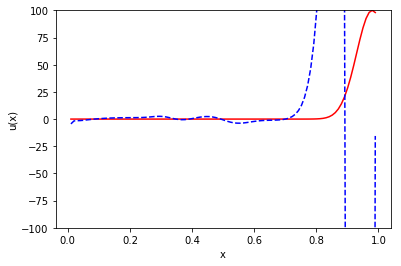
\includegraphics[width = \textwidth]{./functional_sensitivity_figs/pert2.png}
		\subcaption{}
	\end{subfigure}
	\begin{subfigure}[t]{0.4\textwidth}
		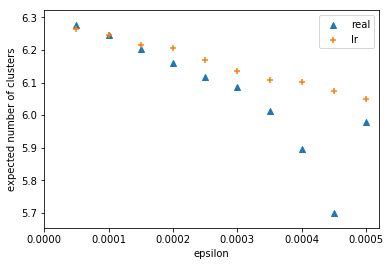
\includegraphics[width = \textwidth]{./functional_sensitivity_figs/vary_epsilon_e_num_clust2.png}
		\subcaption{}
	\end{subfigure}
	\caption{(a) The functional perturbation $u(x)$ that we applied to the prior stick distribution in solid red. The dashed
	blue line is the total influence on the expected number of clusters. (b) Comparing the expected number of clusters gotten from
	re-optimizing with the perturbation $u(x)$ (blue triangles) against the prediction of linear response (orange +), as
	the size of the perturbation $\epsilon$ is varied}
	\label{fig:influence_on_num_clusters2}
\end{figure}


\subsection{Worst-case functional perturbation}
We wish to consider the worst-possible case for a choice of perturbation
$u(\theta)$ \cite{giordano_2017}.
We need some notion of size of perturbation. In our case, we take
\begin{align}
	\|u(\theta)\|_2 := \Big(\int \Big(\frac{u(\theta)}{p_0(\theta)}\Big)^2 p_0(\theta) \; d\theta\Big)^{1/2}
\end{align}
The worst case sensitivity is then defined as
\begin{align}
	S_{sup}^q(\delta) := \sup_{u(\theta) : \|u(\theta)\|_2 \leq \delta} |S_u^q|
\end{align}
and is given by,
\begin{align}
	S_{sup}^q(\delta) = \delta \cdot \text{max} \Big\{\Big(\int|I^+(\theta)|^2p_0(\theta)\; d\theta\Big)^{1/2},
	\Big(\int|I^-(\theta)|^2p_0(\theta)\;d\theta\Big)^{1/2} \Big\}
\end{align}
Let $I^*(\theta)$ be either $I^+(\theta)$, or $I^-(\theta)$, depending on
which attains the max above. Then the worst-case perturbation $u^*(\theta)$
is given by
\begin{align}
	u^*(\theta) = \frac{|I^*(\theta)| p_0(\theta)}{\|I^*(\theta)\|_2}
\end{align}

We consider the worst-case influence perturbation specifically for the sensitivity
of the expected number of posterior clusters. Recall the influence function plotted in
figure \ref{fig:influence_fun_on_num_clusters}b. We compute $u^*(\theta)$ for this
influence function, and this $u^*(\theta)$ is displayed in figure \ref{fig:worst_case_num_clust}.

\begin{figure}[h!]
	\centering
	\begin{subfigure}[t]{0.4\textwidth}
		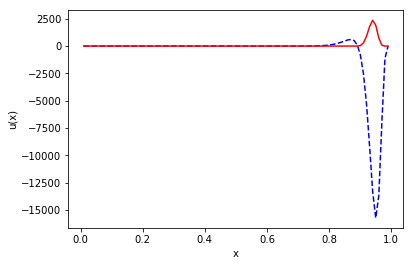
\includegraphics[width = \textwidth]{./functional_sensitivity_figs/worst_case_influence.png}
		% \subcaption{}
	\end{subfigure}
	\caption{The worst case perturbation $u^*(\theta)$ in red; the influence function on the
	expected number of posterior clusters is shown in dashed blue. }
	\label{fig:worst_case_num_clust}
\end{figure}

{\color{red} Perturb by this $u^*(\theta)$ and re-optimize. }

\newpage
\section{Data Sensitivity}
\label{sec:data_sens}
We can also apply the same linear response formulae to approximate perturbations to the dataset. Suppose we augment the
likelihood with weights $w = (w_1, ..., w_n)$ on each datapoint,
\begin{align}
  p(y | \theta, w) = \sum_{n=1}^{n} w_n \; p(y_n | \theta)
\end{align}
And for any positive, finite value of $w$, we can compute
\begin{align}
  \eta^*(w) := \argmin_\eta KL(q_\eta(\theta) \| p(\theta| y, w))
\end{align}
Define $w_1 := (1, ... 1)$, so $\eta^*(w_1)$ is the original variational
posterior. By setting $w$ to other integer-valued vectors, we can produce the
effect of removing or repeating datapoints. In particular, to evaluate
how our posterior results change across bootstrap samples, we can
draw
$w_b \sim Multinomial(n, n^{-1})$ and evaluate $\eta^*(w_b)$. Such a bootstrap
procedure is often employed to evaluate the stability of our results; one hopes
that the clusterings obtained would not change significantly
from bootstrap sample to bootstrap sample.

However, evaluating each bootstrap sample involves re-optimizing for
$\eta^*$, which is computationally expensive. We therefore, can apply
the same linear response ideas as before to approximate perturbations in the
data.  We seek
\begin{align}
  S_w := \frac{d\eta^*(w)}{dw}\Big|_{w = w_1}
\end{align}
so we can approximate
\begin{align}
  \eta^*(w_b) \approx \eta^*(w_1) + S_w(w_b - w_1) \label{eq:bs_lin_approx}
\end{align}
Going through the same derivation that gave rise to equation \ref{eq:vb_sensitivty},
we obtain
\begin{align}
  S_w = - H^{-1} \frac{\partial^2 KL(\eta, w)}{\partial \eta\partial w}\Big|_{w = w_1}
\end{align}

\subsection{Results}
% In figure \ref{fig:bs_vs_lr_diff}a we plot the bootstrapped values $\eta^*(w_b)$ by obtained by the linear
% approximation (equation \ref{eq:bs_lin_approx}), against the bootstrap value obtained
% from re-optimizing. In figure \ref{fig:bs_vs_lr_diff}b we make the same comparison, but
% for the differences $\eta^*(w_b) - \eta^*(w_1)$. There seem to be some differences that are not
% captured by the linear approximation.

To evaluate stability across bootstrap samples, we use two measures of cluster similarity,
the Fowlkes-Mallows score, and and the mutual information score. Let $\phi_{fm}(\eta(w_b))$ and
$\phi_{mi}(\eta(w_b))$ denote the cluster similarity measure obtained by the Fowlkes-Mallows score
and the mutual information score (\cite{fm_score}, \cite{mi_score}), respectively, between the current bootstrap sample $w_b$ and the original
result at $w_1$. To measure the stability of our results,
we seek the distribution of $\phi(\eta^*(w_b))$, with
$w_b \sim Multinomial(n_b, n_b^{-1})$. We approximate this by substituting our linear approximation
for $\eta^*(w_b)$
\begin{align}
  \phi(\eta^*(w_b)) \approx \phi\Big(\eta^*(w_1) + S_w(w_b - w_1)\Big) =: \phi_{lin}(w_b)
  \label{eq:bs_fm_approx}
\end{align}

The distributions of our linear approximation $\phi_{lin}(w_b)$ and the true bootstrap value $\phi(w_b)$
is shown in the bottom row of figure \ref{fig:bs_vs_lr_diff}; the top
row of of figure \ref{fig:bs_vs_lr_diff} compares the predicted values for each bootstrap sample.
We see that the linear bootstrap over-estimates
the similarity of the bootstrap results to the original result.
This is akin to what we observed in figure \ref{fig:vary_alpha_cocluster_weights},
where the linear bootstrap underestimates the change in parameters after
perturbations, as the size of the perturbation gets large.

\begin{figure}[h!]
	\centering
  \begin{subfigure}[t]{0.4\textwidth}
		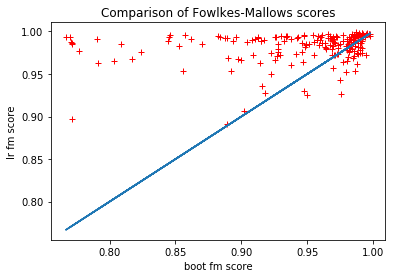
\includegraphics[width = \textwidth]{./data_sens_figs/compare_fm_score.png}
		\subcaption{}
	\end{subfigure}
  \begin{subfigure}[t]{0.4\textwidth}
    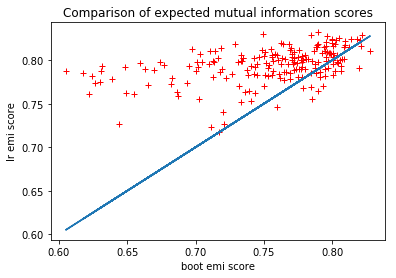
\includegraphics[width = \textwidth]{./data_sens_figs/compare_emi_score.png}
    \subcaption{}
  \end{subfigure}\\
	\begin{subfigure}[t]{0.4\textwidth}
		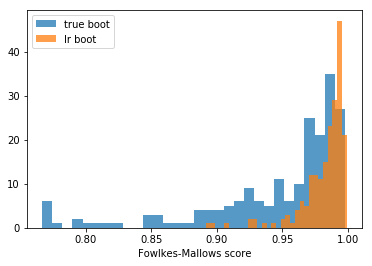
\includegraphics[width = \textwidth]{./data_sens_figs/hist_fm_score.png}
		\subcaption{}
	\end{subfigure}
	\begin{subfigure}[t]{0.4\textwidth}
		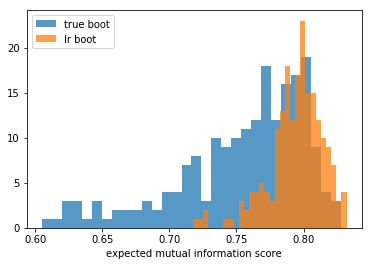
\includegraphics[width = \textwidth]{./data_sens_figs/hist_emi_score.png}
		\subcaption{}
	\end{subfigure}
	\caption{{\bf Top row}: For 200 bootstrap samples $w_b$, we plot the similarity score
	$\phi(\eta^*(w_b))$ obtained by our linear approximation against
  the value obtained after re-optimizing. (a) compares the Fowlkes-Mallows similarity score,
	while (b) uses the expected mutual information score.\\
	{\bf Bottom row}: The distribution of the (c) Fowlkes-Mallows score and (d) the expected mutual information score, as obtained by
  the full bootstrap (blue) and our linear approximation (orange). Here, we computed $\eta^*(w_b)$ in the full bootstrap
  by initializing from
  the original optimum, $\eta^*(w_1)$. }
  \label{fig:bs_vs_lr_diff}
\end{figure}


\section{Comparison with a finite mixture model}
In the previous sections, we used a BNP prior, which allowed us to forgo choosing the number of clusters.
Here, we wish to compare the results obtained from using this BNP prior with results obtained by fitting a
finite mixture model. A common procedure to choose the number of clusters is the model explorer algorithm proposed by
Ben-Hur \cite{model_explorer}, where bootstrap samples are used in same way as in the previous section
to evaluate the examine the stability of the clustering results.
The number of clusters is chosen by seeing which choice gives rise to the most stable clusterings.

The results of this procedure are displayed in figure \ref{fig:finite_mixture_model_explorer} (blue lines),
where we look at the
distribution of cluster similarities across bootstrap samples for various choices
of the number of clusters. We observe that 3 clusters seems to be a reasonable choice.

We can also apply the same linear response techniques to the finite mixture model, and approximate the bootstrap distribution.
The results of the linear bootstrap are shown by the orange lines in \ref{fig:finite_mixture_model_explorer}.
While we see that the linear bootstrap over-estimates the stability scores (like in the results of section \ref{sec:data_sens}),
we again conclude that $k = 3$ is a good choice for the number of clusters. Hence, in this case, the linear
approximation provided an efficient alternative to re-optimizing for every bootstrap sample,
and the resultant choice of $k$ was the same.

\begin{figure}[h!]
	\centering
  \begin{subfigure}[t]{0.4\textwidth}
		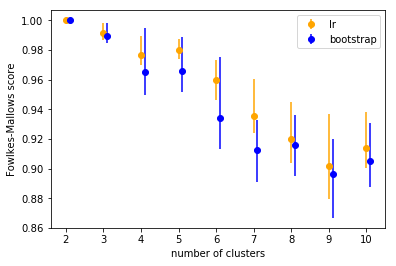
\includegraphics[width = \textwidth]{./finite_mixture_figures/model_explorer_fm_scores.png}
		\subcaption{}
	\end{subfigure}
  \begin{subfigure}[t]{0.4\textwidth}
    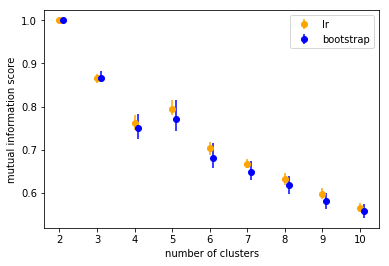
\includegraphics[width = \textwidth]{./finite_mixture_figures/model_explorer_mi_scores.png}
    \subcaption{}
  \end{subfigure}
	\caption{The distribution of the Fowlkes-Mallows score (a) and the mutual information score (b) across bootstrap
  samples, as the number of clusters varies. Blue are distributions obtained from the true bootstrap,
	and red are distributions obtained by our linear approximation. Lines mark the interquartile range. }
  \label{fig:finite_mixture_model_explorer}
\end{figure}

We now use $k = 3$ in the finite mixture model and compare the fits with the BNP model in figures
\ref{fig:BNP_vs_FMM_coclustering} and \ref{fig:cluster_centroids}. We see that
both models give very similar co-clusterings (figure \ref{fig:BNP_vs_FMM_coclustering});
their centroids and cluster covariances are similar as well (figure  \ref{fig:cluster_centroids}).

\begin{figure}[h!]
	\centering
  \begin{subfigure}[t]{0.3\textwidth}
		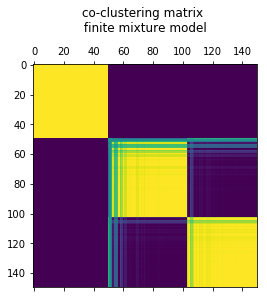
\includegraphics[width = \textwidth]{./finite_mixture_figures/finite_k3_coclust.png}
		\subcaption{}
	\end{subfigure}
  \begin{subfigure}[t]{0.3\textwidth}
    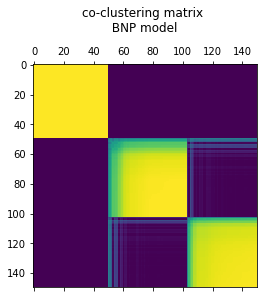
\includegraphics[width = \textwidth]{./finite_mixture_figures/bnp_coclust.png}
    \subcaption{}
  \end{subfigure}
	\caption{(a) the co-clustering matrix obtained using the finite mixture model. (b) the co-clustering matrix
  obtained using the BNP model. Note that each row/column index correspond to the same datapoint in both matrices (i.e. the
  same permutation of rows/columns used to generate plot (a) is the same permutation used then to generate plot (b)).}
  \label{fig:BNP_vs_FMM_coclustering}
\end{figure}

\begin{figure}[h!]
	\centering
  \begin{subfigure}[t]{0.4\textwidth}
		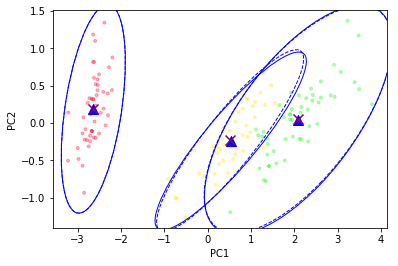
\includegraphics[width = \textwidth]{./finite_mixture_figures/bnp_vs_fin_centroids.png}
	\end{subfigure}
	\caption{Comparing the fits of the BNP model and the finite mixture model. An ``X'' marks the
	BNP centroids, while a triangle marks the finite mixture model centroids;
	dashed blue curves are covariances from the BNP model, while
	solid blue are covariances from the finite mixture model.  }
  \label{fig:cluster_centroids}
\end{figure}



\begin{thebibliography}{9}
\bibitem{model_explorer}
Ben-Hur A, Elisseeff A, and Guyon I. 2001. A stability based method for discovering structure
in clustered data. \textit{In Pacific symposium on biocomputing.}

\bibitem{iris_dataset}
Fisher R. A. 1936. The use of multiple measurements in taxonomic problems.
\textit{Annals of Eugenics.} 7(2): 179–188.

\bibitem{giordano_2017}
Giordano R, Broderick T, and Jordan  M I. 2017.
\textit{Covariances, Robustness, and Variational Bayes}.
\url{https://arxiv.org/abs/1709.02536}.

\bibitem{fm_score}
E. B. Fowlkes and C. L. Mallows. A method for comparing two hierarchical clusterings.
\textit{Journal of the American Statistical Association}.
\url{http://www.jstor.org/stable/2288117}.

\bibitem{mi_score}
Nguyen X V, Epps J, and Bailey J. 2010. Information theoretic measures for clusterings
comparison: Variants, properties, normalization and correction for chance.
\textit{Journal of Machine Learning Research}. 11:2837–2854.

\bibitem{dp_prior}
Sethuraman J. 1994. A constructive definition of dirichlet priors.
\textit{Statistica sinica}. 639–650.

\end{thebibliography}

\end{document}
